\documentclass{article}
\usepackage[utf8]{inputenc}
\usepackage{amsmath}
\usepackage{amsfonts}
\usepackage[margin=0.7in]{geometry}
\usepackage{graphicx}
\usepackage{amssymb}
\usepackage{gensymb}
\usepackage{booktabs}
\usepackage{wrapfig}
\usepackage{caption}
\usepackage[export]{adjustbox}
\usepackage[pdfborder={0 0 0}]{hyperref}
\usepackage{pdfpages}
\usepackage{fancyhdr}
\usepackage{parskip}
\usepackage{lastpage}
\usepackage{listings}
\usepackage{multirow}
\usepackage{xifthen}
\usepackage{xcolor}
\graphicspath{{Images/}} 
\pagestyle{fancy}
\renewcommand{\headrulewidth}{opt}
\title{Programmering og problemløsning, Aflevering 1}
\date{September 2022}
\author{Carl-Emil Rohde}

\usepackage{natbib}

\begin{document}
\maketitle
\section*{Problemformuleringer}
\subsection*{1i0}
Modificer koden angivet i opgaven, så programmet beder brugeren om at angive et programmeringssprog, i stedet for et tal. Når brugeren skriver fSharp, skal programmet returnere teksten: "fSharp is cool". For alle andre Input, skal programmet returnere "I dont know (brugerens input)". Når brugeren skriver "quit", skal programmet stoppe.
\subsection*{1i1}
Lav et program hvor en sort kasse på en hvid baggrund, kan rykkes til højre og venstre ved brug af brugerens input fra højre og venstre piltast. Fra hvert hjørne af canvasset, skal sorte streger forbindes til hver af kassens 4 hjørner. 
\section*{Løsninger og overvejser}
\subsection*{1i0}
Det første jeg ønsker programmet skal gøre når det køres, er at bede brugeren om at indtaste navnet på et programmeringssprog. Dette har jeg gjort ved først at definere en rekursiv funktion (da processen skal ku' gentages), hvorefter jeg har benyttet printfn kommandoen. Herefter har jeg ladet a knytte sig til hvad end brugeren indtaster, ved hjælp a "let"- og "System.Console.readLine" kommandoen. Dernæst har jeg blot matchet a med hhv. "fSharp", "quit" og et wildcard, dvs alt andet end fSharp og quit. Hvis a matcher med fSharp, skriver programmet "fSharp is cool" med en printfn kommando. Matcher a med quit, stopper programmet, da jeg her ved brug af to tomme parenteser (), har valgt at intet skal ske. matcher a med wildcardet, skriver programmet at det ikke kender inputtet. Herefter gentages programmet.
\subsection*{1i1}
I denne del af opgaven, har jeg taget udgangspunkt i koden fra demoprogrammet "MySecondReact.fsx" fundet i src-mappen på absalon. Koden indholder et program, hvor en blå kasse kan rykkes fra side til side med piltasterne. Herfra har jeg modificeret koden, så kassen først og fremmest er sort, og dernæst tilføjet de 4 streger fra hvert hjørne ned til kassen. For at gøre dette, har jeg benyttet kommandoen "do SetLine" og valgt hvilke koordinater stregerne skal gå til og fra.
\subsection*{Billed af færdigt program:}
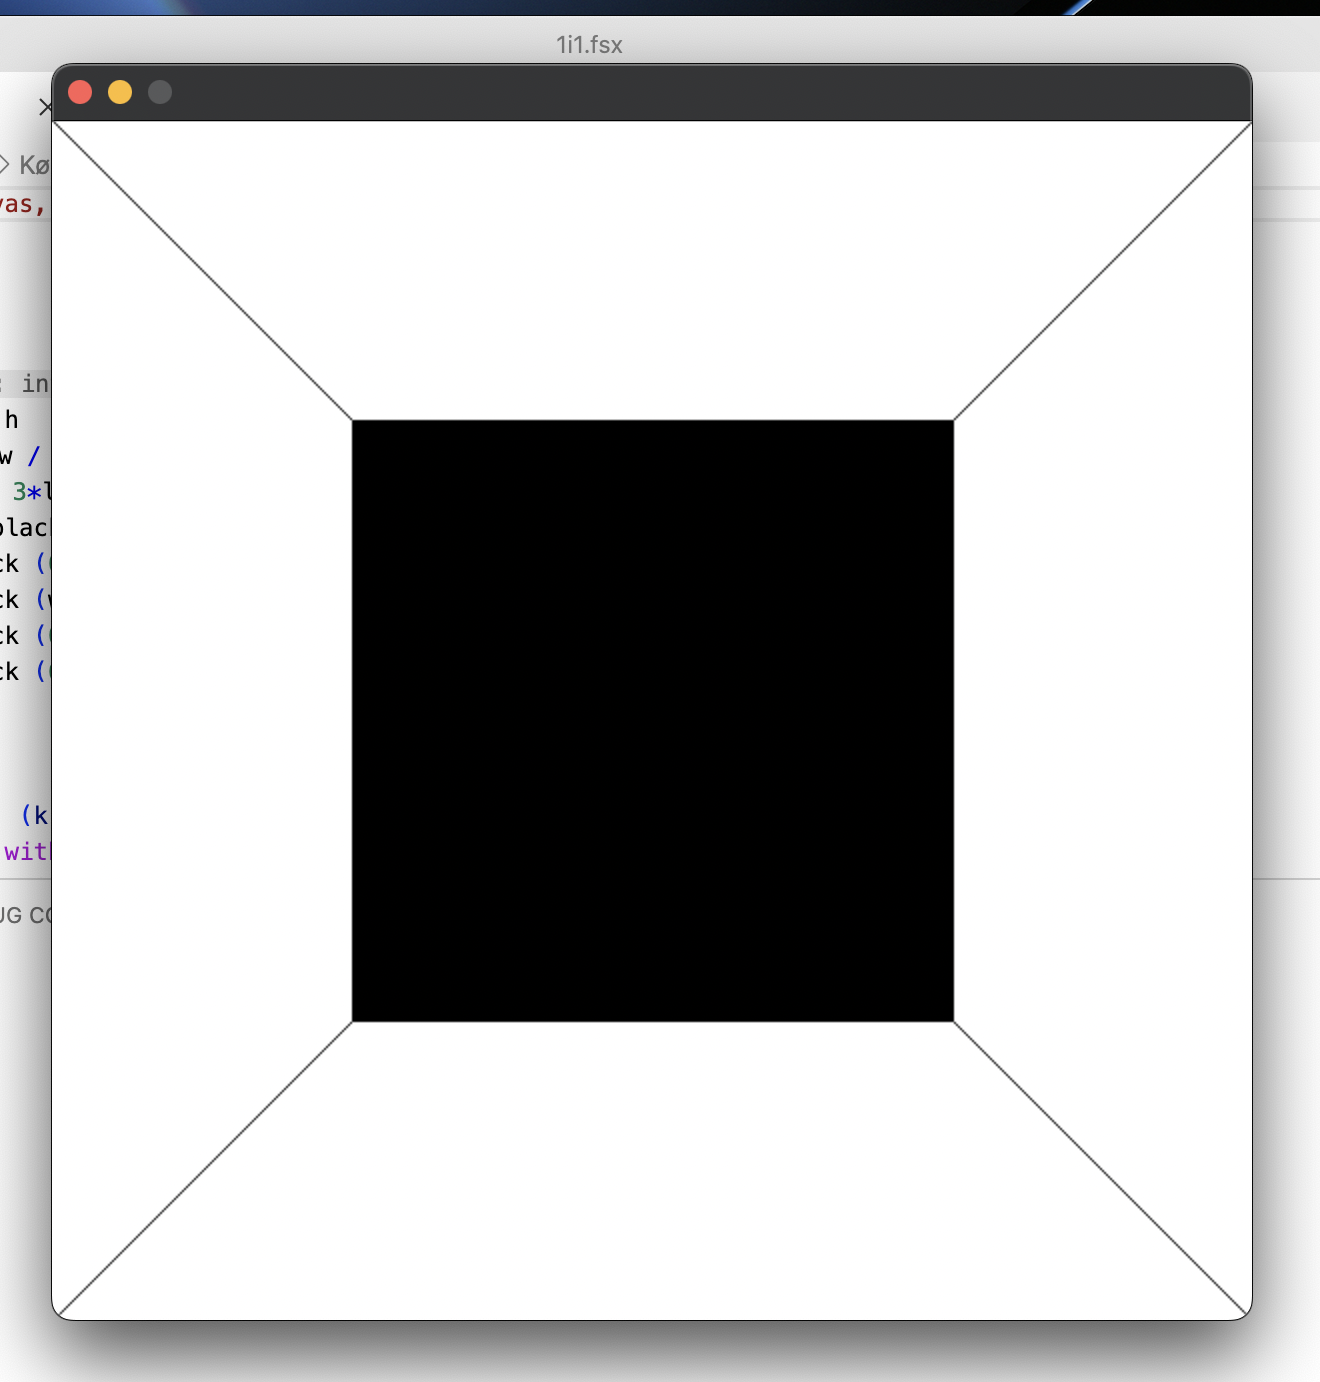
\includegraphics[scale=0.4]{1i1.png}
\end{document}
